\documentclass{beamer}
\mode<presentation>
\usepackage{amsmath}
\usepackage{amssymb}
%\usepackage{advdate}
\usepackage{adjustbox}
\usepackage{subcaption}
\usepackage{enumitem}
\usepackage{multicol}
\usepackage{mathtools}
\usepackage{listings}
\usepackage{url}
\def\UrlBreaks{\do\/\do-}
\usetheme{Boadilla}
\usecolortheme{lily}
\setbeamertemplate{footline}
{
  \leavevmode%
  \hbox{%
  \begin{beamercolorbox}[wd=\paperwidth,ht=2.25ex,dp=1ex,right]{author in head/foot}%
    \insertframenumber{} / \inserttotalframenumber\hspace*{2ex} 
  \end{beamercolorbox}}%
  \vskip0pt%
}
\setbeamertemplate{navigation symbols}{}

\providecommand{\nCr}[2]{\,^{#1}C_{#2}} % nCr
\providecommand{\nPr}[2]{\,^{#1}P_{#2}} % nPr
\providecommand{\mbf}{\mathbf}
\providecommand{\pr}[1]{\ensuremath{\Pr\left(#1\right)}}
\providecommand{\qfunc}[1]{\ensuremath{Q\left(#1\right)}}
\providecommand{\sbrak}[1]{\ensuremath{{}\left[#1\right]}}
\providecommand{\lsbrak}[1]{\ensuremath{{}\left[#1\right.}}
\providecommand{\rsbrak}[1]{\ensuremath{{}\left.#1\right]}}
\providecommand{\brak}[1]{\ensuremath{\left(#1\right)}}
\providecommand{\lbrak}[1]{\ensuremath{\left(#1\right.}}
\providecommand{\rbrak}[1]{\ensuremath{\left.#1\right)}}
\providecommand{\cbrak}[1]{\ensuremath{\left\{#1\right\}}}
\providecommand{\lcbrak}[1]{\ensuremath{\left\{#1\right.}}
\providecommand{\rcbrak}[1]{\ensuremath{\left.#1\right\}}}
\theoremstyle{remark}
\newtheorem{rem}{Remark}
\newcommand{\sgn}{\mathop{\mathrm{sgn}}}
\providecommand{\abs}[1]{\left\vert#1\right\vert}
\providecommand{\res}[1]{\Res\displaylimits_{#1}} 
\providecommand{\norm}[1]{\lVert#1\rVert}
\providecommand{\mtx}[1]{\mathbf{#1}}
\providecommand{\mean}[1]{E\left[ #1 \right]}
\providecommand{\fourier}{\overset{\mathcal{F}}{ \rightleftharpoons}}
%\providecommand{\hilbert}{\overset{\mathcal{H}}{ \rightleftharpoons}}
\providecommand{\system}{\overset{\mathcal{H}}{ \longleftrightarrow}}
	%\newcommand{\solution}[2]{\textbf{Solution:}{#1}}
%\newcommand{\solution}{\noindent \textbf{Solution: }}
\providecommand{\dec}[2]{\ensuremath{\overset{#1}{\underset{#2}{\gtrless}}}}
\newcommand{\myvec}[1]{\ensuremath{\begin{pmatrix}#1\end{pmatrix}}}
\let\vec\mathbf

\lstset{
%language=C,
frame=single, 
breaklines=true,
columns=fullflexible
}

\numberwithin{equation}{section}

\title{Presentation Template}
\author{Sri Sathwik Desaboina \\ AI24BTECH11007}

\date{\today} 
\begin{document}

\begin{frame}
\titlepage
\end{frame}

\section*{Outline}
\begin{frame}
\tableofcontents
\end{frame}
\section{Problem}
\begin{frame}
\frametitle{Problem Statement}
%

Show that the point $\myvec{x \\ y}$ given by $x = \frac{2at}{1 + t^2}$ and $y = \frac{a(1 - t^2)}{1 + t^2}$ lies on a circle for all real values of $t$ such that $-1 \leq t \leq 1$, where $a$ is any given real number.
\end{frame}

%\subsection{Literature}
\section{Solution}
\subsection{Usage of variables}
\begin{frame}
\frametitle{Usage of variables}
	\begin{tabular}[12pt]{ |c| c| c|}
    \hline
    \textbf{S.No} & \textbf{variables used}&\textbf{description}\\ 
    \hline
	$1$ & \textit{t} & a variable which takes the real values in the range $(-1,1)$\\
    \hline
	$2$ & \textit{a} & it is a fixed real number \\
    \hline
	$3$ & $\vec{A(t)}$ & it is a transformation matrix of parameter t\\
    \hline
	$4$ & $\vec{v(t)}$ & it represent the parameter t and allows to define x and y \\
    \hline
	$5$ & $\vec{p(t)}$ & a point with coordinates x and y. \\
    \hline
    \end{tabular}

\end{frame}
\subsection{Parametric form}
\begin{frame}
\frametitle{Parametric form}
Given $x$ and $y$ in the parametric form,\\
	\begin{align}
		x &= \frac{2at}{1 + t^2},\\
		\quad y &= \frac{a(1 - t^2)}{1 + t^2}
	\end{align}
	Let $\vec{p(t)}$ be equal to,\\
	\begin{align}
	\mathbf{p}(t) = \myvec{x \\ y} = \myvec{\frac{2at}{1 + t^2} \\ \frac{a(1 - t^2)}{1 + t^2}}.
	\end{align}


\end{frame}
\subsection{Matrix equation}
\begin{frame}
\frametitle{Matrix equation}
	The transformation matrix $\vec{A(t)}$ and $\vec{v(t)}$ with parameter $t$ are,\\
	\begin{align}
		\implies \mathbf{A}(t) & = \myvec{ \frac{2a}{1+t^2} & 0 \\ 0 & \frac{a(1-t^2)}{1+t^2}},\\ \implies \mathbf{v(t)} &= \myvec{t \\ 1},\\ \mathbf{p(t)} &= \mathbf{A(t)} \mathbf{v(t)}, \\\implies  \mathbf{p}(t) & = \myvec{ \frac{2a}{1+t^2} & 0 \\ 0 & \frac{a(1 - t^2)}{1+t^2} } \myvec{t \\ 1},\\ 
	\end{align}
\end{frame}
%\section{Plot}
\subsection{Verification}
\begin{frame}[fragile]
\frametitle{Verification}
Now, if we check the value of ,
    \begin{align}
    \mathbf{p}(t)\top \myvec{ 1 & 0 \\ 0 & 1 } \mathbf{p}(t)
    \end{align}
	We get,\\
  \begin{align}
    \mathbf{p}(t)\top \myvec{ 1 & 0 \\ 0 & 1 } \mathbf{p}(t)=a^2
    \end{align}

	$\implies$ We proved that the given points lie on a circle $x^2 + y^2 = a^2$.\\
	Since we have the values of $t$ in $(-1,1)$, the y-coordinate of the points is always positive.\\
	We get a semi-circle with those points.

The codes for verification:
 {\footnotesize
\begin{lstlisting}
https://github.com/DESABOINASRISATHWIK/EE1030/blob/main/presentation/codes/plot.py
https://github.com/DESABOINASRISATHWIK/EE1030/blob/main/presentation/codes/code.c
\end{lstlisting}}


\end{frame}
\subsection{Plot}
\begin{frame}
	\frametitle{Plot}
\begin{figure}[h!]
    \centering
    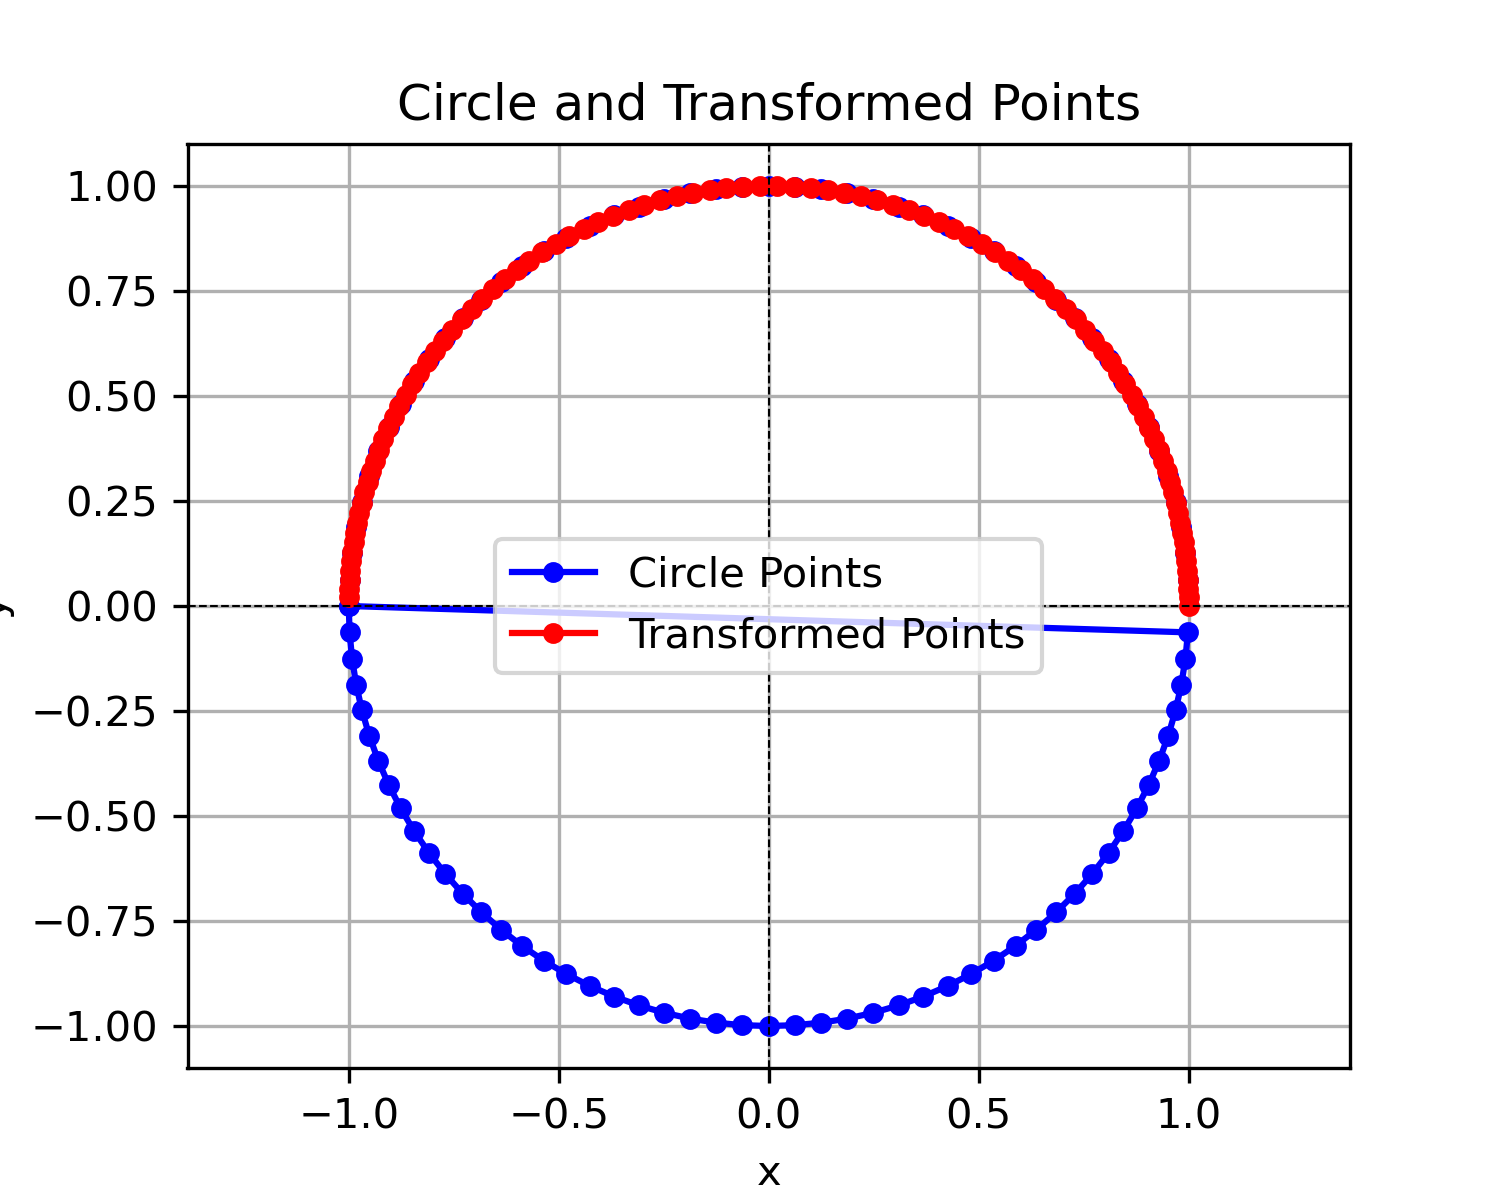
\includegraphics[width=0.8\textwidth]{figs/plot.png} 
    \caption{Circle Points}
    \label{fig:circle_plot}
\end{figure}

\end{frame}
\end{document}
